\documentclass[justified]{tufte-handout}
\usepackage{../braph2_tut}
%\geometry{showframe} % display margins for debugging page layout

\title[Analysis and Comparison of Memory Capacity WU]{Pipeline for Analysis Comparison of Memory Capacity using Weighted Undirected Graph}

\begin{document}

\maketitle

\begin{abstract}
\noindent
This tutorial shows how to perform a \emph{reservoir computing} analysis using \emph{connectivity data} (see tutorial \href{https://github.com/braph-software/BRAPH-2/tree/develop/tutorials/data/tut_gr_con}{Group of Subjects with Connectivity Data}), where one connectivity matrix per subject is available, as in diffusion weighted imaging or pre-calculated matrices obtained from functional MRI, MEG, or EEG. Step by step, this pipeline guides you to first analyze the data of a group of subjects and then compare the data from two groups of subjects, were matrices are \emph{weighted undirected}.  With this tutorial, you will be able to extract and plot differences between two groups. You will also be able to generate publication-quality figures.
\end{abstract}

\tableofcontents

\clearpage
\section{Generate Example Data}

You can generate the example data by typing in the command line the instruction in \Coderef{cd:generate}.

\begin{lstlisting}[
	label=cd:generate,
	caption={
		{\bf Command to generate example data.}
		Command to generate the example data for connectivity analyses. This script will create two groups of subjects and the associated atlas files. Each subject has a weighted random connectivity matrix with a mean nodal degree of 4, which has been derived using the Watts–Strogatz model (group 1 uses a rewiring probability of 0.3 and group 2 has a rewiring probability of 0.85). After running the code, the data will be created in \fn{.braph2memorycapacity/pipelines/memorycapacity/Example Data memory capacity}, and includes the brain atlas \fn{atlas.xlsx}, two folders with the subject files \fn{MC\_Group\_1\_XLS} and \fn{MC\_Group\_2\_XLS}, and the associated covariates files \fn{MC\_Group\_1\_XLS.vois.xlsx} and \fn{MC\_Group\_2\_XLS.vois.xlsx}. The details about the format of these files can be found in the tutorials \href{https://github.com/braph-software/BRAPH-2/tree/develop/tutorials/data/tut_ba}{Brain Atlas} and \href{https://github.com/braph-software/BRAPH-2/tree/develop/tutorials/data/tut_gr_con}{Group of Subjects with Connectivity Data}.
	}
	]
	create_data_memorycapacity()
\end{lstlisting}

\section{Open the GUI}

The GUI of BRAPH~2 Memory Capacity Distribution can be opened by typing \code{braph2} in MatLab's terminal. This GUI allows you to select a pipeline, as shown in \Figref{fig:01}.

%! FIG1 !%
\fig{figure}
{fig:01}
{
	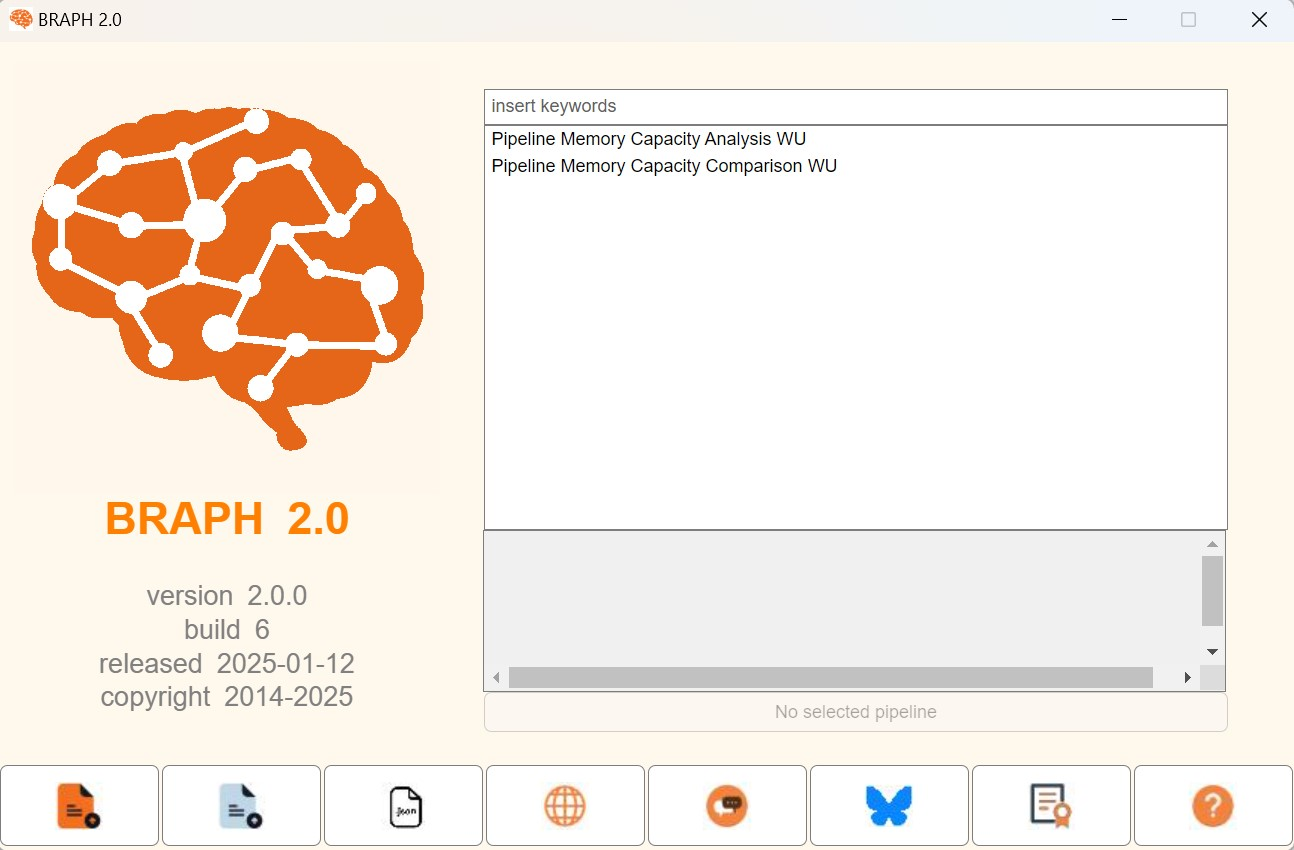
\includegraphics{fig01.jpg}
}
{BRAPH~2 Memory Capacity Distribution main GUI}
{
	BRAPH~2 main GUI with the two pipelines for this distribution: \emph{Pipeline Memory Capacity Analysis WU} and \emph{Pipeline Memory Capacity Comparison WU}.
}
In this tutorial it will be explained \emph{Pipeline Memory Capacity Comparison WU} since it also covers \emph{Pipeline Memory Capacity Analysis WU} (Step 3 and Step 4 of the tutorial). First, we select the pipeline that we want to run. Once a it is selected a short description of the pipeline will be displayed, as shown in \Figref{fig:02}. Then we press the \fn{Open Pipeline Memory Capacity Comparison WU} button.

%! FIG2 !%
\fig{figure}
{fig:02}
{
	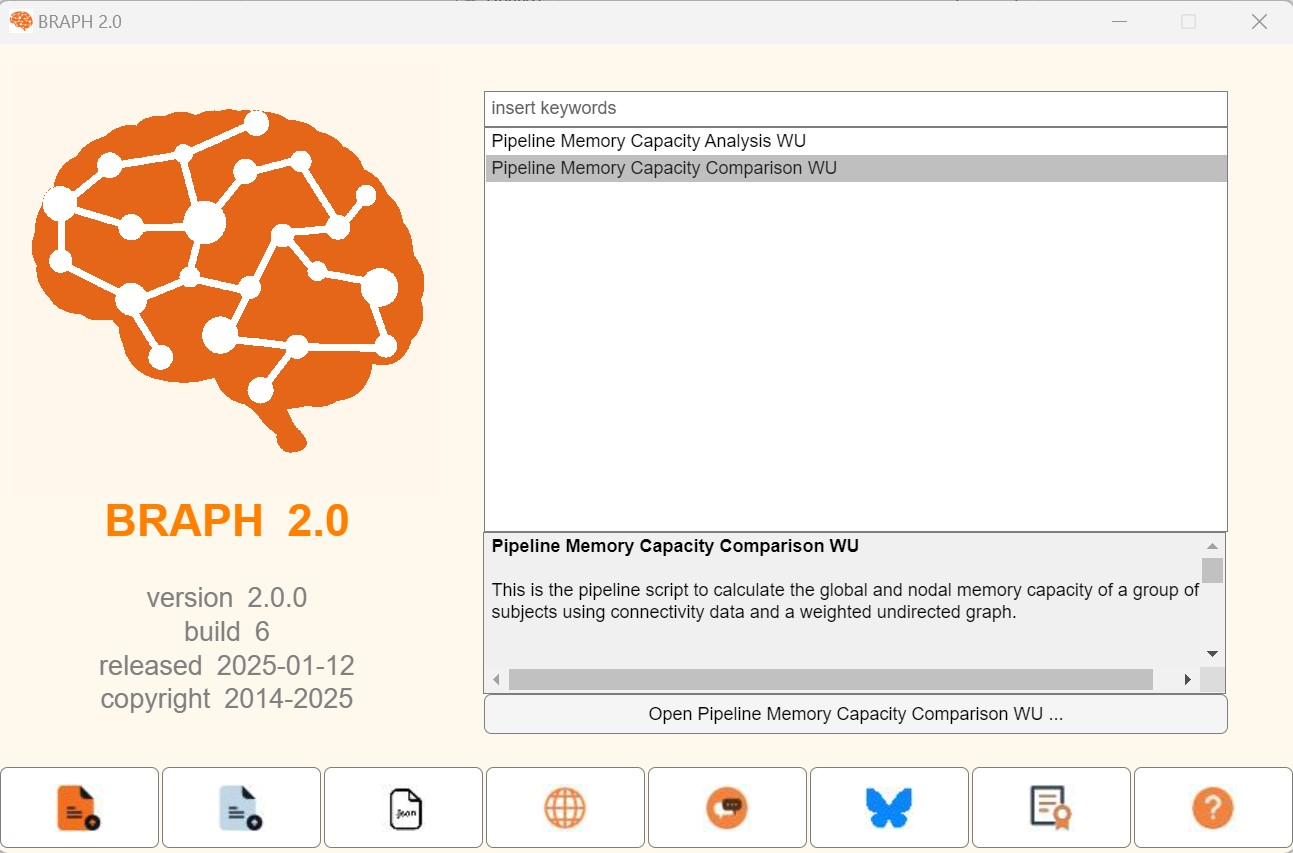
\includegraphics{fig02.jpg}
}
{Pipeline Memory Capacity Comparison WU}
{
	Selected \emph{Pipeline Memory Capacity Comparison WU} with short description.
}

Once the pipeline is uploaded, you can see a GUI that contains different steps to: upload a brain atlas, upload the connectivity data of two groups, analyze them, and finally, compare the groups (\Figref{fig:03}). 

\fig{marginfigure}
{fig:03}
{
	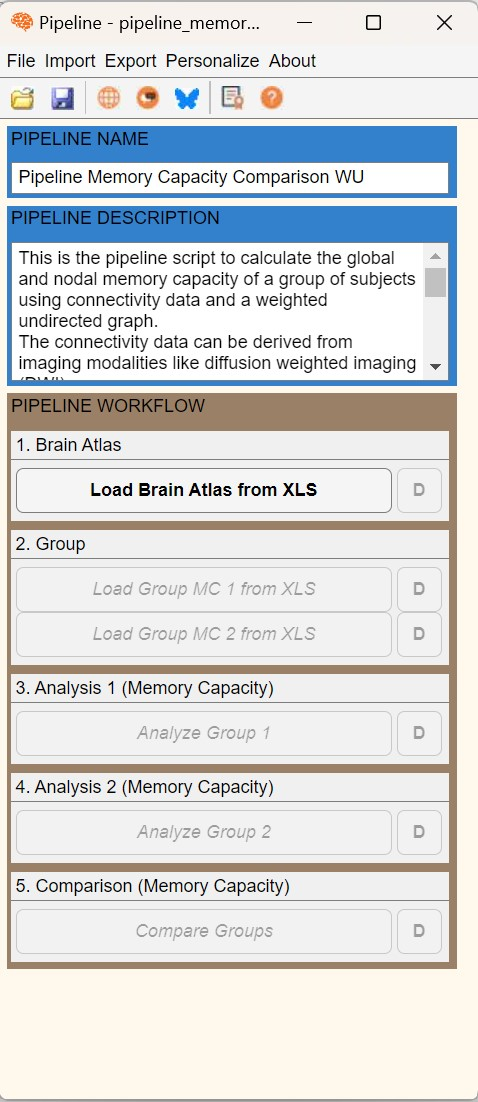
\includegraphics{fig03.jpg}
}
{Pipeline steps}
{
	These are the steps of the pipeline. Only the first step is active when the pipeline is first opened. Subsequent steps will become active sequentially.
}

\clearpage
\section{Step 1: Load the Brain Atlas}


\Figref{fig:04} shows how to upload and plot the brain atlas that you used to extract the data for your analysis. For more information on where to find different atlases or how to change plotting settings on the brain surface, check the tutorial \href{https://github.com/braph-software/BRAPH-2/tree/develop/tutorials/data/tut_ba}{Brain Atlas}.

\fig{figure*}
{fig:04}
{
	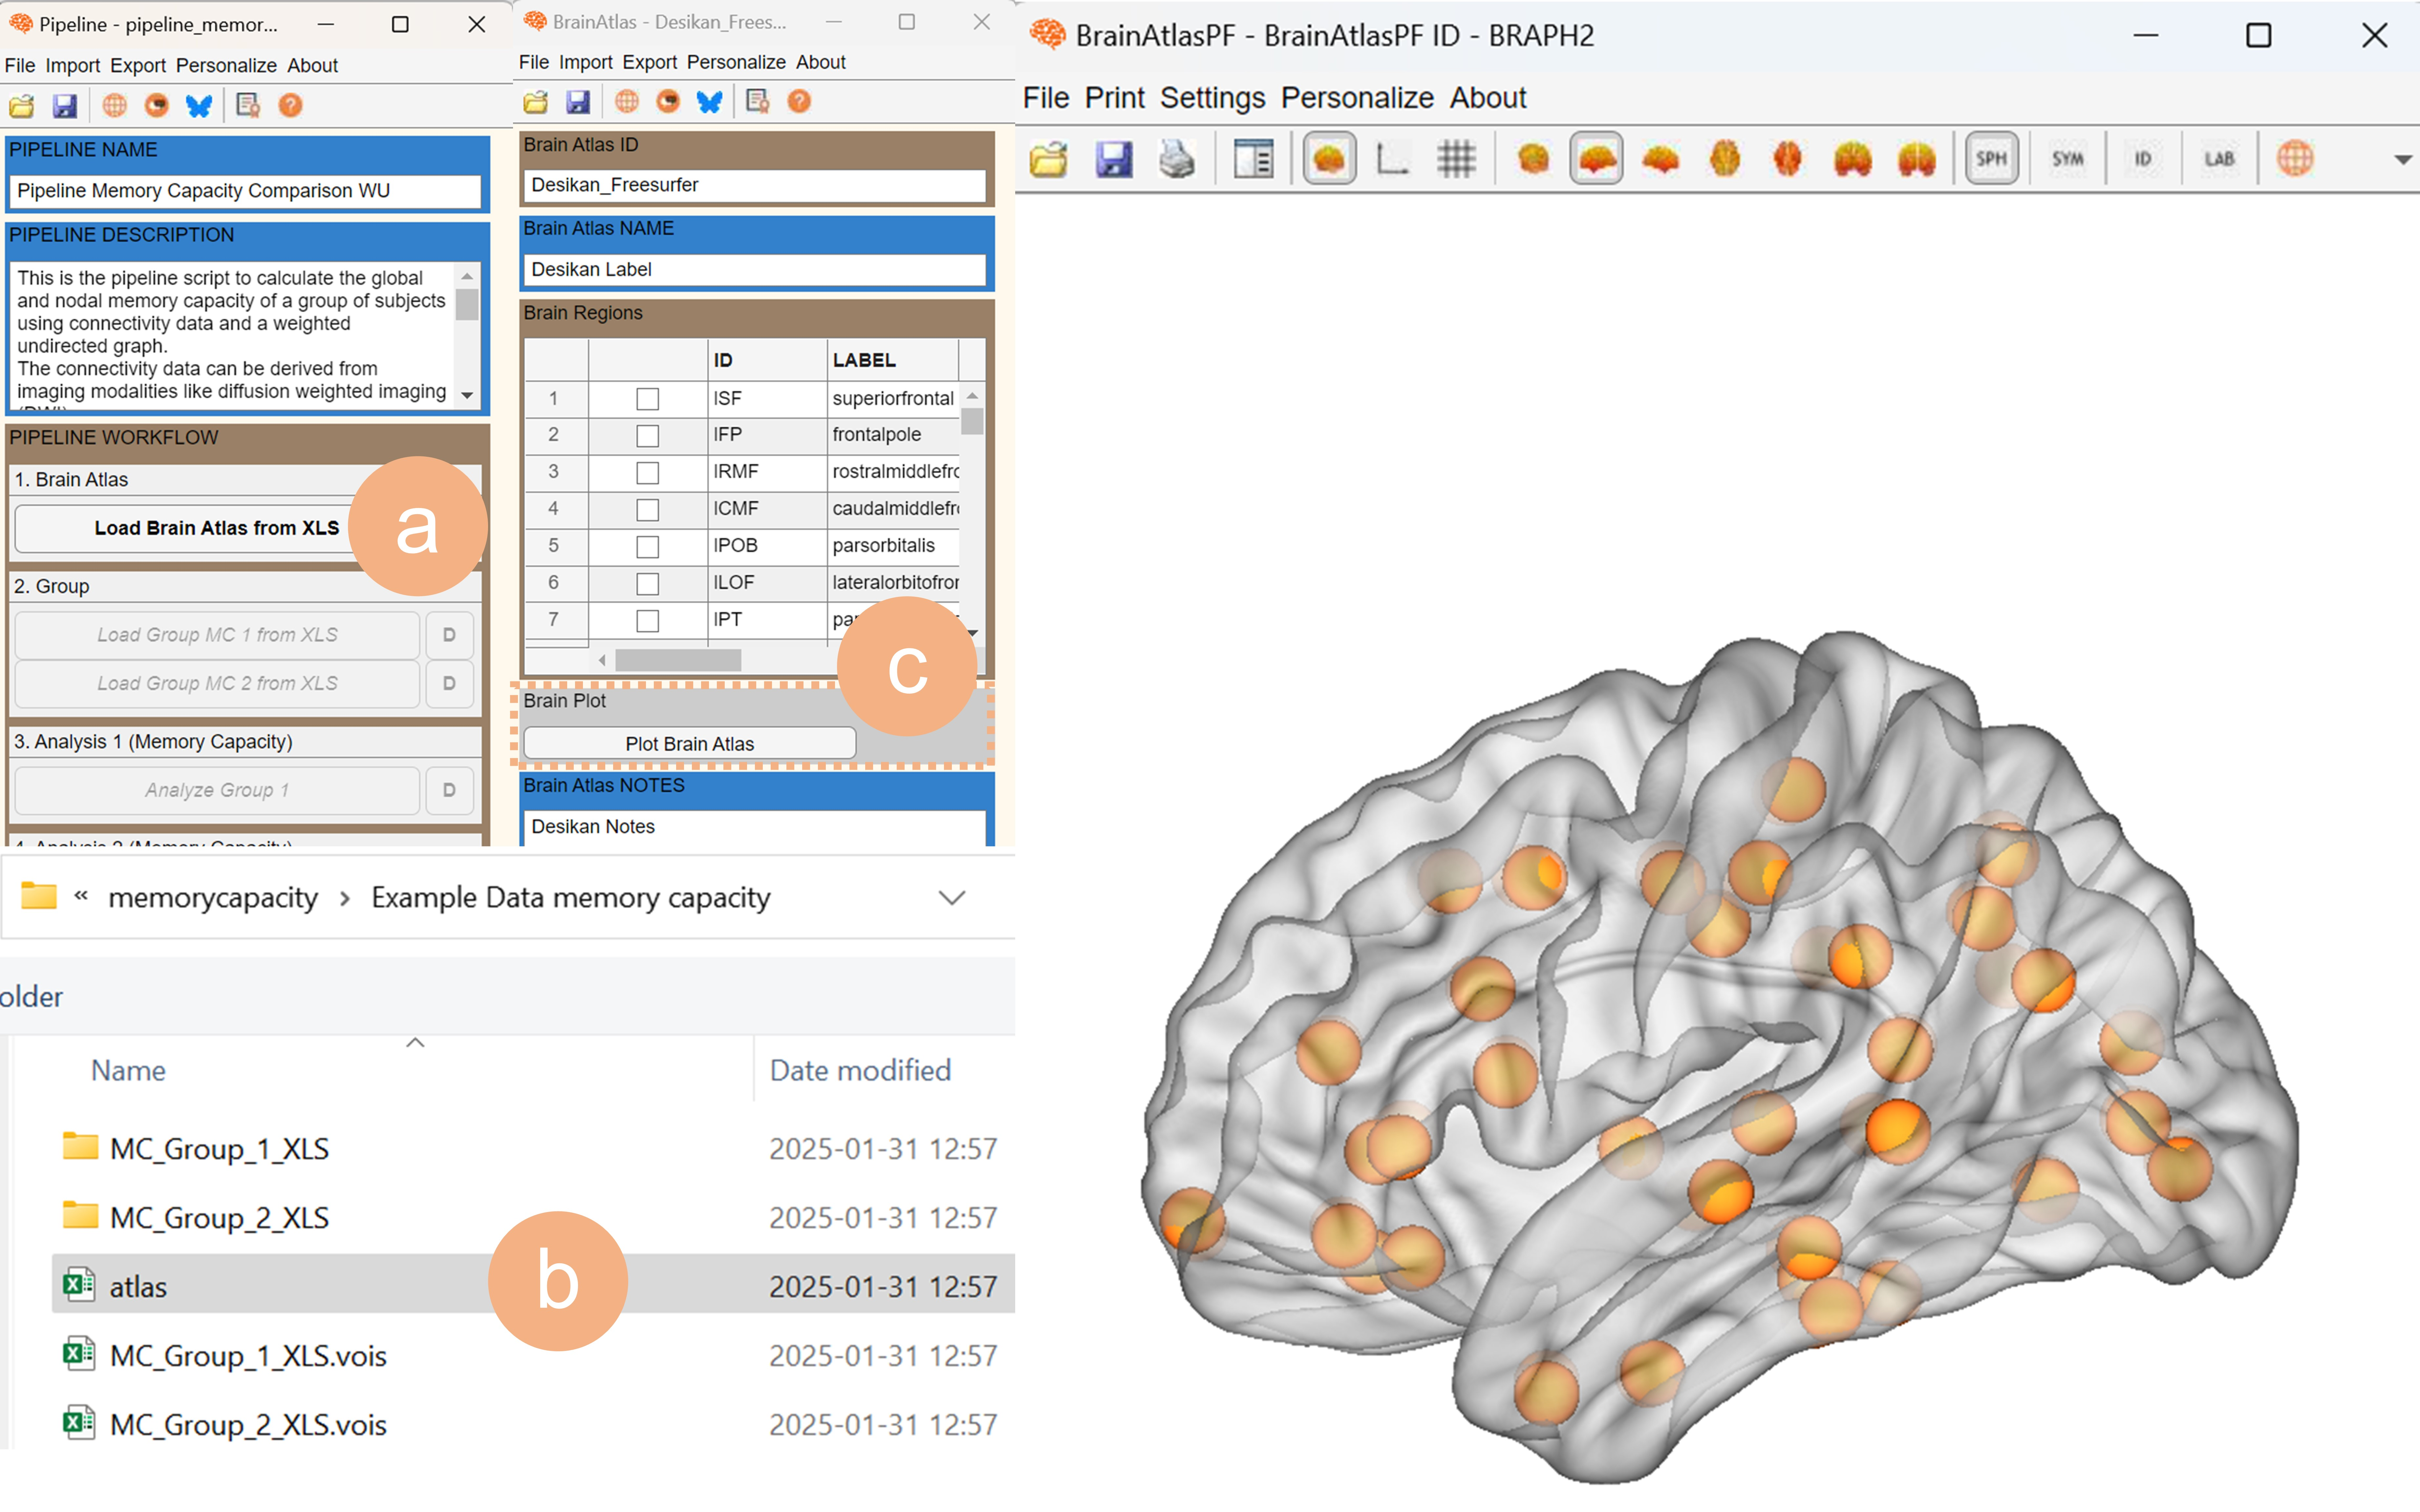
\includegraphics{fig04.jpg}
}
{Uploading the Brain Atlas}
{
	Steps to upload the brain atlas:
	{\bf a} Click on \fn{Load Atlas} from the pipeline GUI.
	{\bf b} Navigate to the BRAPH~2 folder \fn{atlases} or the \emph{Example Data memory capacity folder} and select one of the atlas files, in this example the \fn{atlas.xlsx}. 
	{\bf c} You can visualize the brain atlas by pressing \fn{Plot Brain Atlas}. 
}

\clearpage
\section{Step 2: Load the Connectivity Group Data}

After you have loaded the brain atlas, you can upload the \emph{connectivity data} for each group as shown in \Figref{fig:05}. A new interface will be shown containing the data for the group you just selected. You can open each subject’s connectivity matrices by selecting the subject, right click, and select “Open selection” (for more information check the tutorial \href{https://github.com/braph-software/BRAPH-2/tree/develop/tutorials/data/tut_gr_con}{Group of Subjects with Connectivity Data}).

\fig{figure*}
{fig:05}
{
	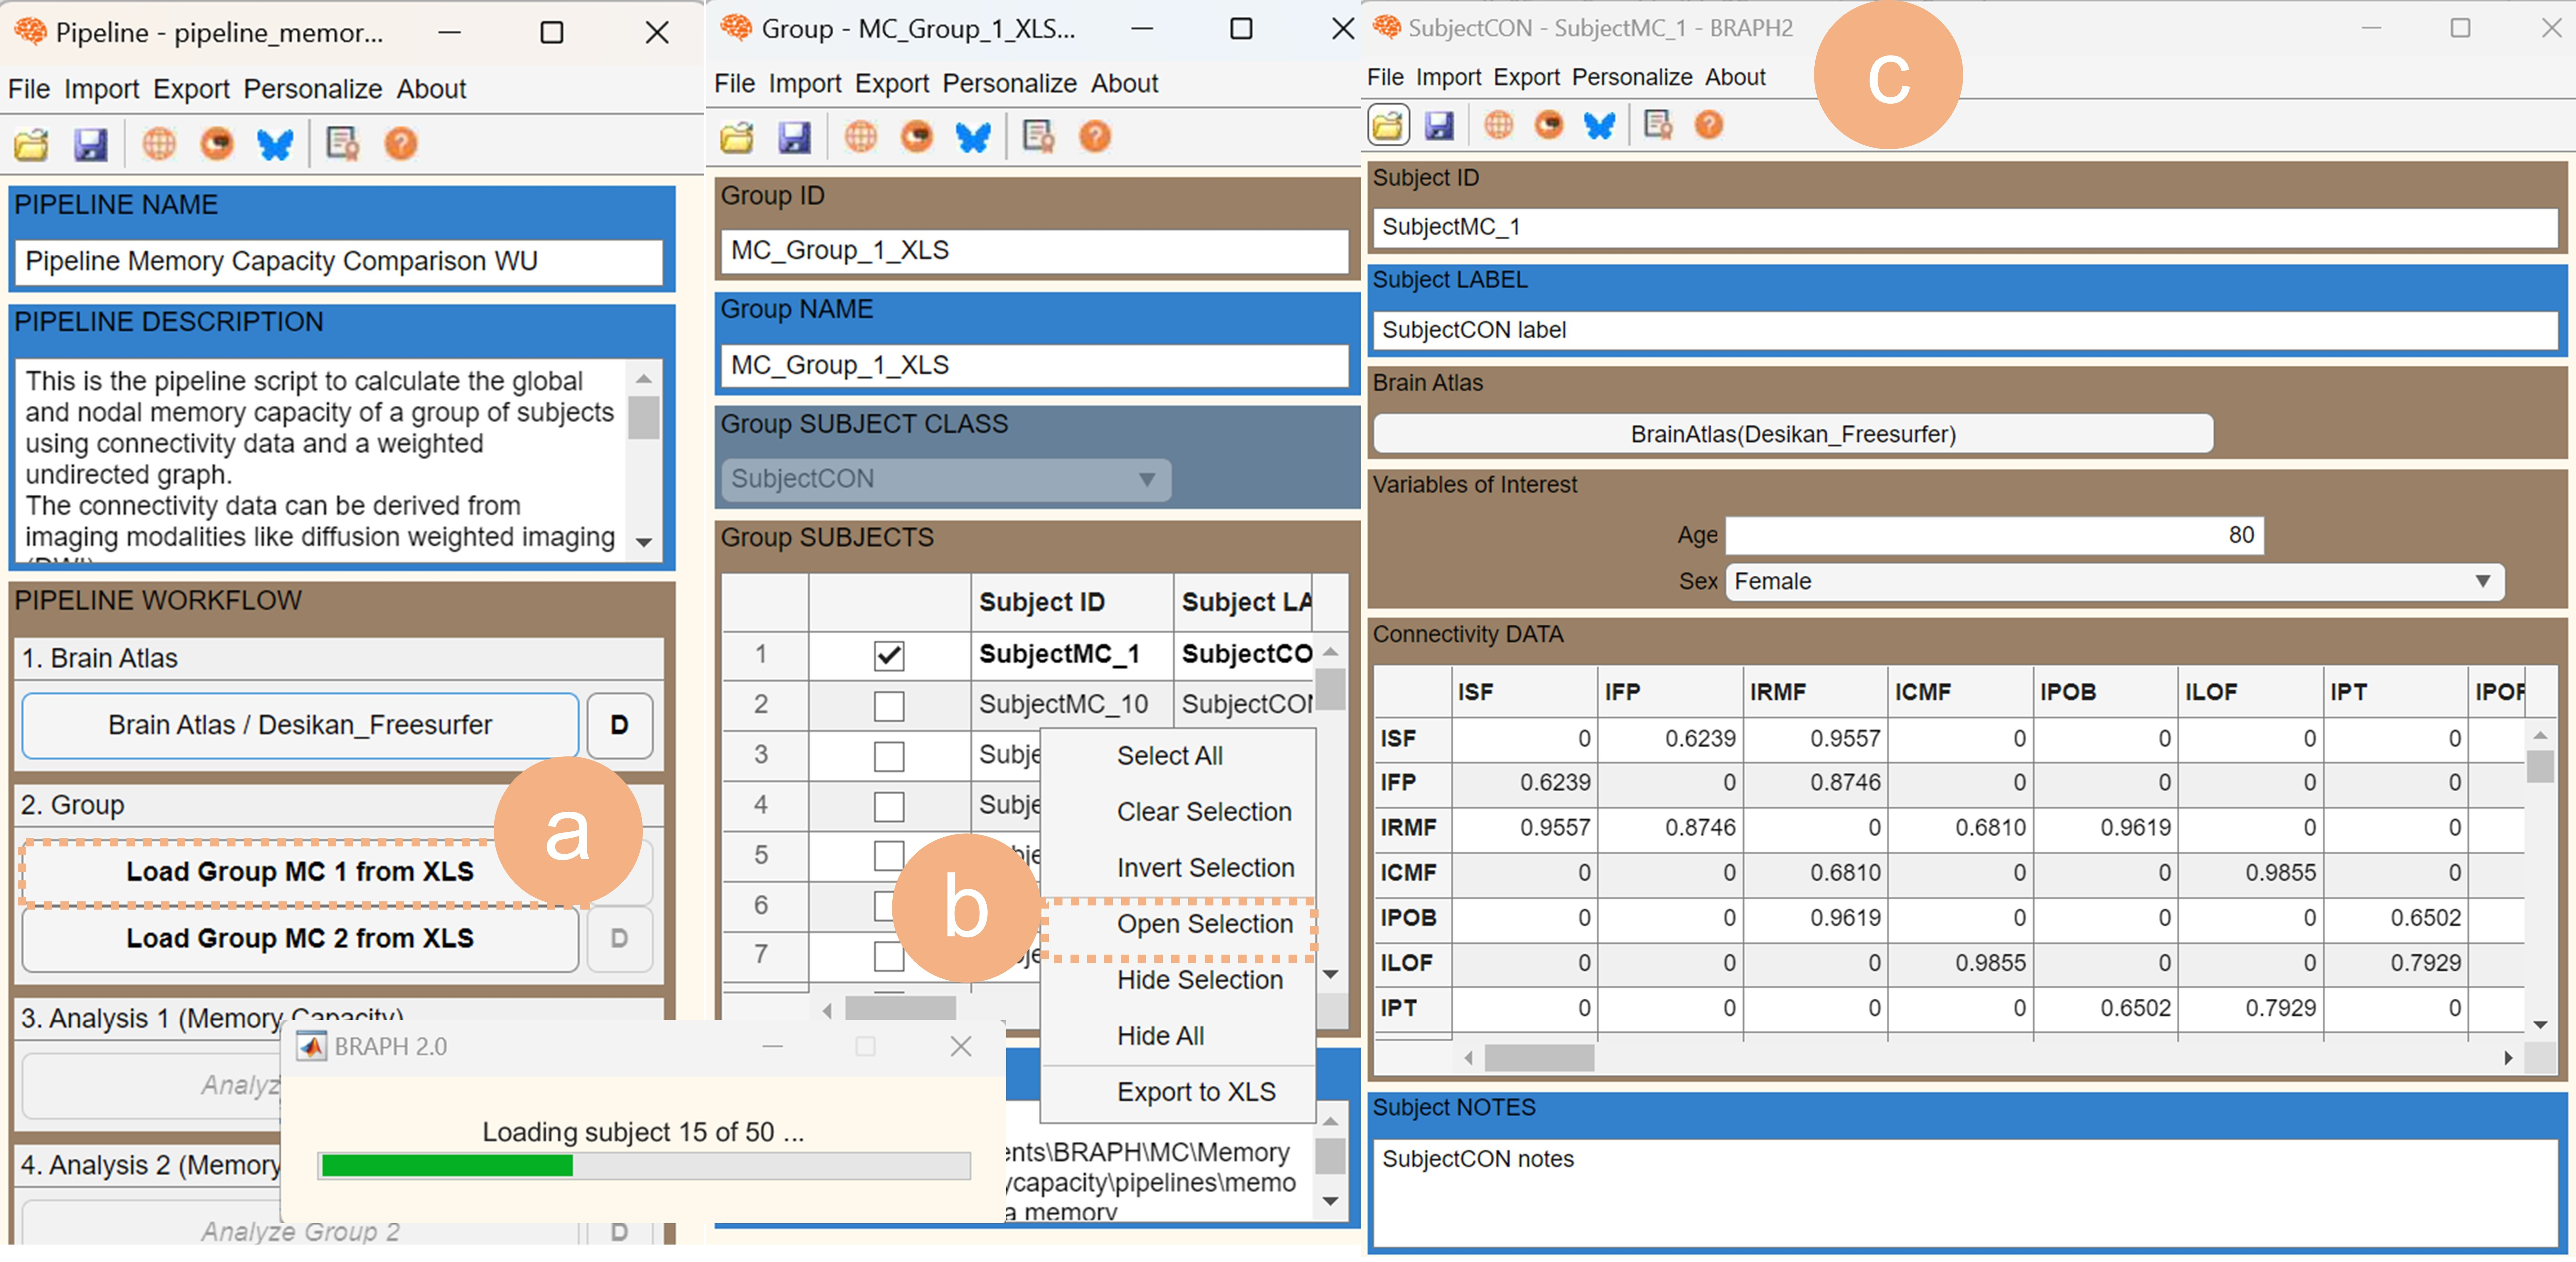
\includegraphics{fig05.jpg}
}
{Loading and visualizing the group data}
{
	{\bf a} From the pipeline GUI, click on \fn{Load Group CON 1 from XLS} to load the data of group 1.
	{\bf b} Once the data is uploaded, you can select a subject, right click and select \code{Open selection}.
	{\bf c} This will open the connectivity matrix of the subject in addition to the age and sex of that subject (which are the variables of interest available for the example data).
	You can then repeat the same procedure for group 2.
}


%! FIG5 !%

\clearpage
\section{Step 3: Analyzing the Data of Group 1}


\subsection{Setting Analysis Parameters}



\subsection{Setting Graph Parameters}


\subsection{Setting Measure Parameters}


\clearpage
\subsection{Calculate Measures}

%! FIG9 !%


\section{Step 4: Analyzing the Data of Group 2}



\clearpage
\section{Step 5: Comparing Groups}





\end{document}